\newpage
\subsection{UC4 - Modifica Grafico}
\label{sub:uc4}

%TODO: Add correct image
\begin{figure}[h]
    \centering
    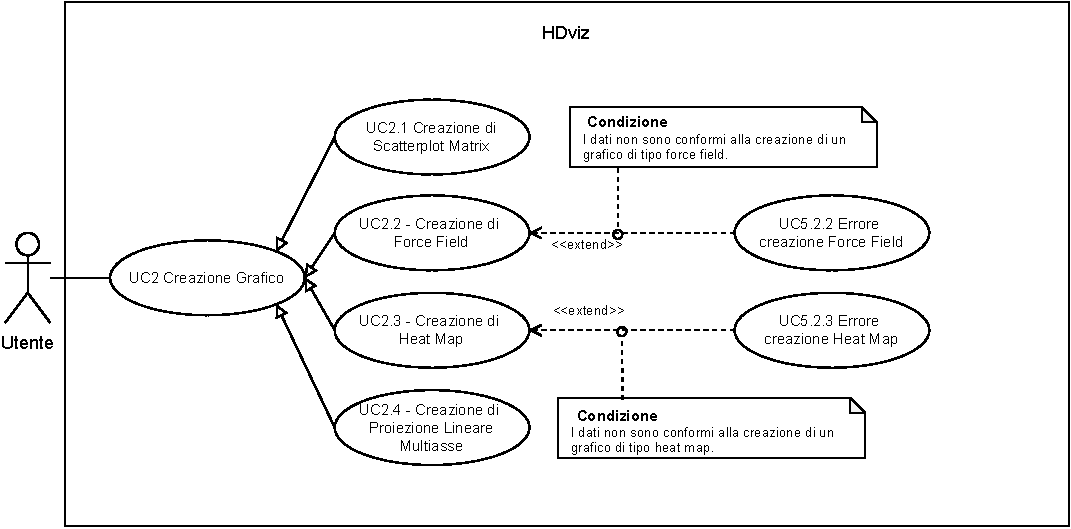
\includegraphics[width=0.8\textwidth]{componenti/casi-duso/diagrammi/UC2.pdf}
    \caption{Diagramma rappresentante UC2}
    \label{fig:UC4}
\end{figure}


\begin{itemize}
    \item \textbf{Descrizione}: L’utente modifica la visualizzazione del grafico precedentemente costruito
                                e ne vede le modifiche.
	
    \item \textbf{Attore primario}: Utente.
    
    \item \textbf{Precondizione}:   Nel programma è stato importato un dataset dotato di metatag per ogni
                                    colonna dei dati ed è stato costruito un grafico di una tipologia scelta dall'utente.

    \item \textbf{Postcondizione}:  Viene aggiornato il grafico costruito e visualizzato con i nuovi parametri.

	\item \textbf{Scenario principale}:
		\begin{enumerate}
			\item L'utente decide di modificare il grafico corrente.
			\item L'utente effettua le modifiche desiderate.
            \item L'utente conferma le modifiche apportate aggiornado il grafico costruito che viene visualizzato.
        \end{enumerate}

    \item \textbf{Generalizzazioni}:
        \begin{itemize}
            \item Modifica del grafico Scatterplot Matrix (UC4.1)
            \item Modifica del grafico Force Field (UC4.2)
            \item Modifica del grafico Heat Map (UC4.3)
            \item Modifica del grafico Proiezione Lineare Multiasse (UC4.4)
        \end{itemize}
\end{itemize}


\subsection{UC4.1 Modifica Scatterplot Matrix}





\subsection{UC4.2 Modifica Force Field}
% TODO: Create image for force field graph.
\begin{figure}[h]
    \centering
    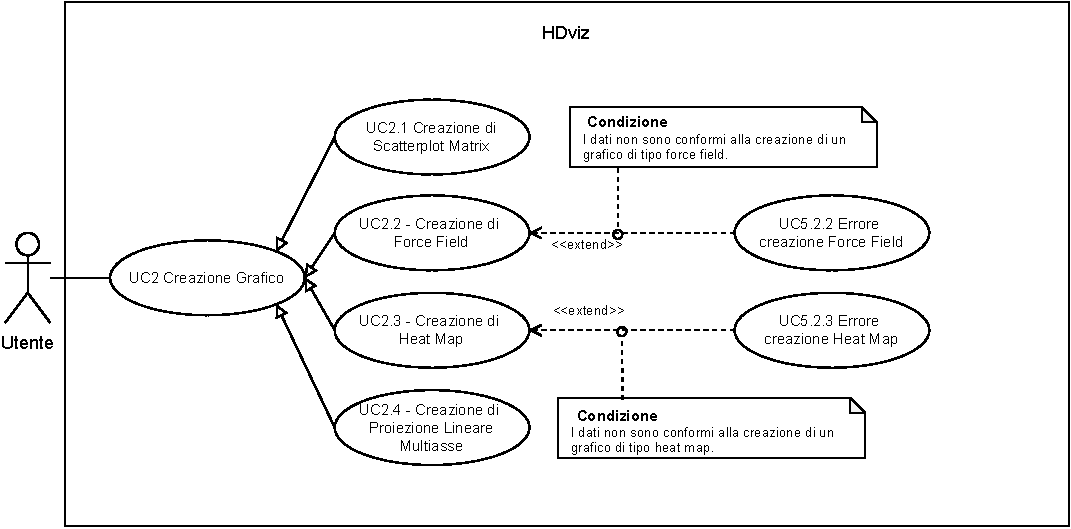
\includegraphics[width=0.8\textwidth]{componenti/casi-duso/diagrammi/UC2.pdf}
    \caption{Diagramma rappresentante UC2}
    \label{fig:UC2}
\end{figure}


\begin{itemize}
    \item \textbf{Descrizione}: L’utente vuole modificare la visualizzazione del grafo Force Field
                                costruito dal dataset corrente.
	
    \item \textbf{Attore primario}: Utente.
    
    \item \textbf{Precondizione}:   Il grafico precedentemente costruito dal dataset corrente è un Force Field.

    \item \textbf{Postcondizione}:  Viene aggiornato il grafico costruito e visualizzato con i nuovi parametri.

	\item \textbf{Scenario principale}:
		\begin{enumerate}
            \item L'utente apporta le modifiche desiderate tra quelle offerte dal Force Field.
        \end{enumerate}
\end{itemize}

\subsubsection{UC4.2.1 Modifica posizione dei nodi}

\begin{itemize}
    \item \textbf{Descrizione}: L’utente vuole modificare la posizione dei nodi del 
                                grafico trascinandoli con il cursore.
	
    \item \textbf{Attore primario}: Utente.
    
    \item \textbf{Precondizione}:   Il grafico precedentemente costruito dal dataset corrente è un Force Field.

    \item \textbf{Postcondizione}:  Viene aggiornato il grafico costruito e visualizzato con i nuovi parametri.

	\item \textbf{Scenario principale}:
        \begin{enumerate}
            \item L'utente tiene premuto e trascina il cursore per spostare il punto nello spazio del grafico.
            \item Il grafico si muove mantentendo le connessioni tra i nodi.
        \end{enumerate}
\end{itemize}

\subsubsection{UC4.2.2 Modifica dell'algoritmo delle distanze}

\subsubsection{UC4.2.3 Modifica intensità forza attrattiva tra nodi}

\subsubsection{UC4.2.4 Modifica di un nodo per dimensione}
